\chapter{Design and Analysis of the Dental Surgical Robot - DentiBot}
\section{Requirement and Specification}
(Payload, resolution and workspace)														\\
(Why not RCM mechanism)																	
\section{Design of the DentiBot}
As discussed in previous section, we have to select correct devices according to those requirement. First, We choose Meca500 manufactured by Mecadamic Inc. as our 6 DOF robot arm. Its feature is high repeatability (precision: 5 $\mu m$) and it is equipped with zero-backlash speed reducers. In addition, it is compact and portable for laboratory investigation. Second, Mini40 manufactured by ATI Inc. is the corresponding F/T sensor with three force and three torque detections. As for the end effector, we modify a existing dental handpiece which equips a tool change mechanism. The modified handpiece weights around 139 grams. We also design  adapters so as to assemble these devices.\\
DentiBot has seven degree of freedom. 6 DOF is come from Meca500, and the other DOF is owing to our modified handpiece. The rotation of root canal file is driven by a servo motor whose maximum rotation speed is more than 600 rpm.																		
\section{Kinematics Analysis}
\label{sec:kinematics}
The purpose of this section and section \ref{sec:ref_robot} is to serve as a tutorial and provide some important approaches when combining a robot arm and an end effector. We derive the forward and inverse kinematics in section \ref{sec:forward} and describe Jacobian matrix in section \ref{sec:jacobian}. 
\subsection{Coordinate Definition}
In Fig \ref{fig:frames} , we define frame\{0\} to frame\{6\} which represent each frame of axis of the Meca500, frame\{S\} which represent the frame of the ATI-mini40 and frame\{H\} which represent the frame of the handpiece.
\begin{figure}[htbp]
\begin{center}
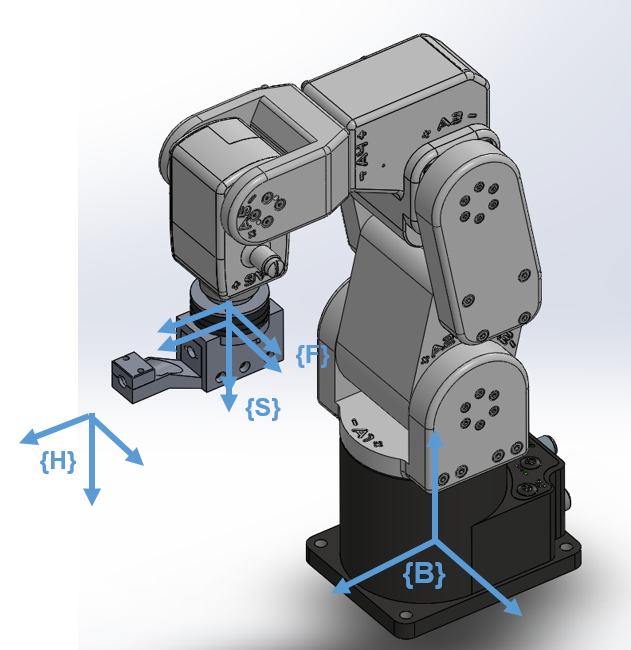
\includegraphics[width=0.8\linewidth]{Images/Coordinates1.png}
\end{center}
\caption{
Coordinate Definition
}\label{fig:frames}
\end{figure} 
\subsection{Forward and Inverse Kinematics}
\label{sec:forward}
\begin{table}[H]
\centering
\caption{Denavit-Hartenberg parameters of Meca500}
\label{tab:DHtable}
\begin{tabular}{ccccc} 
\hline \hline
$i$ (link number)		&$\alpha _{i-1}$ (deg)	&$a_{i-1}$ (mm)	& $\theta _i$ (deg)			&$d_i$ (mm)	\\\hline
1   					&0    					&0				&$\theta _1$				&135 \\
2   					&-90   					&0				&$\theta _2$				&0 \\
3  						&0    					&135			&$\theta _3$ 				&0 \\
4   					&-90    				&38				&$\theta _4$ 				&120 \\
5   					&90   					&0				&$\theta _5$ 				&0 \\
6						&-90  					&0				&$\theta _6$ 				&70 \\
\end{tabular}
\end{table}
Denavit-Hartenberg parameters are shown as Table \ref{tab:DHtable}. Then, the forward kinematics of Meca500 is derived as
\begin{equation*}
\begin{split}
^0_6\text{T} =
\ ^0_1\text{T} \cdot \ ^1_2\text{T} \cdot \ ^2_3\text{T} \cdot \ ^3_4\text{T} \cdot \ ^4_5\text{T} \cdot \ ^5_6\text{T} =
\begin{bmatrix}
^0_6\text{R}_{3\times 3} 	&^0\vec{P}_{6org}\\
0_{1\times 3}				&1\\
\end{bmatrix}
\end{split}
\end{equation*}
where $^0_6\text{R}_{3\times 3}$ is the rotation matrix from frame\{6\} to frame\{0\}, $^0\vec{P}_{6org}$ is the origin of the frame\{6\} observed from frame\{0\}.\\
All detailed indexes of $^0_6\text{T}$ are shown as Appendix \ref{appendix:forward}

\subsection{Jacobian matrix} 
\label{sec:jacobian}
(variables are shown in appendix because they are too long)												\\
(How to obtain Jacobian matrix in frame 6 by Jacobian matrix in frame 0)
\section{Reference Frame Changing of the Robot Arm}
\label{sec:ref_robot}
So far, with forward and inverse kinematics the robot arm can translate and rotate around frame\{6\}. However the origin of the frame\{6\} is not considered to be an operating point. Because the F/T sensor and a detachable end effector will be both mounted on the wrist, the position of the tool tip is exactly what we want. That means we should let the robot arm know how to translate and rotate in frame\{T\} instead of frame\{6\}. If we have translation and rotation information of the tool tip, there is an easy way to directly give these above information to the robot arm. SetTRF (x,y,z,$\alpha$,$\beta$,$\gamma$) is the command of the robot arm, whose (x,y,z) is translation vector and ($\alpha$,$\beta$,$\gamma$) is rotation vector in representation of Euler angle .\\	
In order to obtain translation and rotation vector, we respectively introduce Tool Center Point in section \ref{sec:tcp} to find the translation vector and propose an approach in section \ref{sec:rot inf} to find the rotation vector.							
\subsection{Tool Center Point}
\label{sec:tcp}
Tool Center Point (TCP) is a critical problem for robot arm control. In previous section, we have calculated the forward and inverse kinematics of the robot arm. By Calculating kinematics we can keep track of the origin of the frame\{6\}, which is observed from the base frame. The robot arm has capability to translate and rotate with the origin of the frame\{6\}. These above motions is like a remote center motion (RCM). We should find the position of the tool tip and make it be a RCM point. Nevertheless, it's not efficient to recalculate the transformation matrix via mechanism dimension when changing an end effector or a tool (root canal reamer).\\
To overcome this problem, we demonstrate four-points method to obtain the position of the tool tip which is also the translation vector.\\
From Fig \ref{fig:frames}, we can obtain the following transformation matrix,
\begin{equation}
\begin{split}
_{H}^{B}\textrm{T} &=\  _{F}^{B}\textrm{T}\ _{H}^{F}\textrm{T}\\
\end{split}
\end{equation}		
and it can be rewritten as
\begin{equation}
\begin{split}																												
\begin{bmatrix}
_{H}^{B}\textrm{R} & ^{B}\vec{P}_{H_{org}}\\ 
0 & 1
\end{bmatrix} &=
\begin{bmatrix}
_{F}^{B}\textrm{R} & ^{B}\vec{P}_{F_{org}}\\ 
0 & 1
\end{bmatrix}
\begin{bmatrix}
_{H}^{F}\textrm{R} & ^{F}\vec{P}_{H_{org}}\\ 
0 & 1
\end{bmatrix}\\
%----------------------------------------------------------------------------------------------------------------------------
&= 
\begin{bmatrix}
_{F}^{B}\textrm{R}_{H}^{F}\textrm{R} & _{F}^{B}\textrm{R}^{F}\textrm{P}_{H_{org}} +\ ^{B}\vec{P}_{F_{org}}\\ 
0 & 1
\end{bmatrix}\\
\end{split}
\end{equation}
Therefore, we get a crucial equation:
\begin{equation}
\begin{split}
^{B}\vec{P}_{H_{org}} &=\  _{F}^{B}\textrm{R}\cdot\ ^{F}\vec{P}_{H_{org}} +\ ^{B}\vec{P}_{F_{org}}\\
\end{split}
\end{equation}
Now, we can move the tool tip to a fixed point with four different pose (position and orientation). Then, we will get four different rotation matrix and vectors in real time. 
\begin{equation}
\begin{split}																									
^{B}\vec{P}_{H_{org}} &=\  _{F}^{B}\textrm{R}^{1}\cdot\ ^{F}\vec{P}_{H_{org}} +\ ^{B}\vec{P}_{F_{org}}^{1}\\
%----------------------------------------------------------------------------------------------------------------------------
					  &=\  _{F}^{B}\textrm{R}^{2}\cdot\ ^{F}\vec{P}_{H_{org}} +\ ^{B}\vec{P}_{F_{org}}^{2}\\
%----------------------------------------------------------------------------------------------------------------------------
					  &=\  _{F}^{B}\textrm{R}^{3}\cdot\ ^{F}\vec{P}_{H_{org}} +\ ^{B}\vec{P}_{F_{org}}^{3}\\
%----------------------------------------------------------------------------------------------------------------------------
					  &=\  _{F}^{B}\textrm{R}^{4}\cdot\ ^{F}\vec{P}_{H_{org}} +\ ^{B}\vec{P}_{F_{org}}^{4}\\
%----------------------------------------------------------------------------------------------------------------------------
\end{split}\label{eq:four-points}
\end{equation}
In order to extract $^{F}\vec{P}_{H_{org}}$ from Eq.\ref{eq:four-points}, we subtract the second to forth equation from the first equation.
\begin{equation}
\begin{split}	
\begin{bmatrix}
\  _{F}^{B}\textrm{R}^{1} - \  _{F}^{B}\textrm{R}^{2}\\ 
\  _{F}^{B}\textrm{R}^{1} - \  _{F}^{B}\textrm{R}^{3}\\ 
\  _{F}^{B}\textrm{R}^{1} - \  _{F}^{B}\textrm{R}^{4}
\end{bmatrix}
\cdot\ ^{F}\vec{P}_{H_{org}} 
=
\begin{bmatrix}
\ ^{B}\vec{P}_{F_{org}}^{2} -\ ^{B}\vec{P}_{F_{org}}^{1} \\ 
\ ^{B}\vec{P}_{F_{org}}^{3} -\ ^{B}\vec{P}_{F_{org}}^{1} \\ 
\ ^{B}\vec{P}_{F_{org}}^{4} -\ ^{B}\vec{P}_{F_{org}}^{1} 
\end{bmatrix}
\end{split}
\end{equation}
where
\begin{equation*}
\begin{split}
\textbf{R} =  
\begin{bmatrix}
\  _{F}^{B}\textrm{R}^{1} - \  _{F}^{B}\textrm{R}^{2}\\ 
\  _{F}^{B}\textrm{R}^{1} - \  _{F}^{B}\textrm{R}^{3}\\ 
\  _{F}^{B}\textrm{R}^{1} - \  _{F}^{B}\textrm{R}^{4}
\end{bmatrix}_{9 \times 3}, 
\textbf{P} = 
\begin{bmatrix}
\ ^{B}\vec{P}_{F_{org}}^{2} -\ ^{B}\vec{P}_{F_{org}}^{1} \\ 
\ ^{B}\vec{P}_{F_{org}}^{3} -\ ^{B}\vec{P}_{F_{org}}^{1} \\ 
\ ^{B}\vec{P}_{F_{org}}^{4} -\ ^{B}\vec{P}_{F_{org}}^{1} 
\end{bmatrix}_{9 \times 1}
\end{split}
\end{equation*}
Therefore,
\begin{equation*}
\begin{split}
^{F}\vec{P}_{H_{org}} &= \textbf{R}^{\dagger} \cdot \textbf{P}\\
					  &= \left( \textbf{R}^T\textbf{R}\right) ^{-1}\cdot \textbf{R}^T\cdot \textbf{P}
\end{split}
\end{equation*}
Hence, we can utilize four-points method to obtain the translation vector.
\subsection{Rotation Information}
\label{sec:rot inf}
First, we have to find the vector of tool insertion direction $\vec{t}$. By means of TCP method, we can obtain the translation vector from the origin of frame\{6\} to the tool tip. Therefore we use two root canal files with different lengths and apply TCP method to separately obtain two vector illustrated as Fig . Hence, 
\begin{equation}
\begin{split}
\vec{t} =\ ^{F}\vec{P}_{H_{org},\ long} -\ ^{F}\vec{P}_{H_{org},\ short}
\end{split}
\end{equation}
For analyze it easily, we depict it in Fig \ref{fig:rot_inf}. Note that here we only discuss rotation.
\begin{figure}[htbp]
\begin{center}
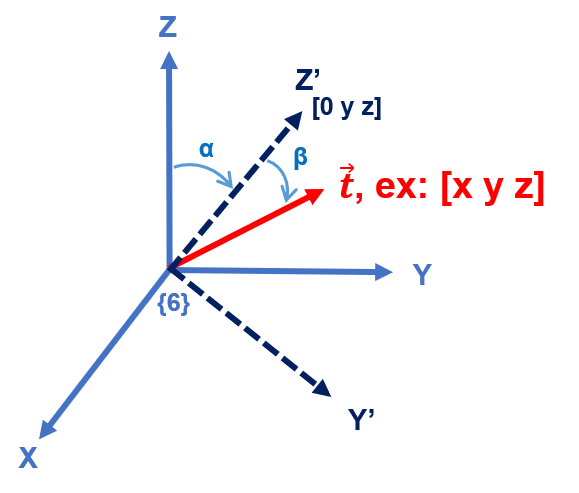
\includegraphics[width=0.6\linewidth]{Images/rot_inf.png}
\end{center}
\caption{
Illustration of finding rotation matrix
}\label{fig:rot_inf}
Because we hope to send z axis command to achieve tool insertion, we should align original Z axis to the target vector. Therefore, Z axis alignment without other restrictions will produce many solutions. We choose one of solutions to align Z axis to the target vector. According to the figure, we assume the target vector is [1,1,1], whose projection to YZ frame is [0,1,1]. First, we rotate $\alpha$ degree around X axis to make original Z axis align the projection [0,1,1]. Next, we rotate $\beta$ degree around Y' axis and finally align original Z axis to the target vector [1,1,1]. 
\begin{equation}
\begin{split}
\ ^T_6R = R_x\left(\alpha \right) R_y\left(\beta \right)  
\end{split}
\end{equation}
where $\alpha$ and $\beta$ are Euler angles, which meet the command demand.
\end{figure} 
We have described two key aspects of reference frame changing of the robot arm. Finally, input the results of section \ref{sec:tcp} and section \ref{sec:rot inf} via the command setTRF to make the robot arm recognize frame\{T\}.